\chapter{\label{chap:evaluation}Evaluation}

In this chapter, the results are examined in closer detail to provide an insight
into the inner working of the algorithms. The questions raised during the course
of the paper are answered, shortcomings and possible improvements are discussed,
and the work is contrasted to pre-existing research. This evaluation is
performed for each of the three phases of the pipeline:
\begin{itemize}
    \item Raster Exclusion Using \blobdog{} (in Section~{\ref{sec:eval-dog}})
    \item Ant Colony (in Section~\ref{sec:eval-ant})
    \item Gravitational Clustering (in Section~\ref{sec:eval-clustering})
\end{itemize}

\section{\label{sec:eval-dog}Raster Exclusion Using \blobdog{}}

\paragraph{What is the behavior displayed by \blobdog{}?}\paragraphnewline{}
\noindent To examine the behavior of \blobdog{}, results for various rasters across the
areas are displayed in Figure~\ref{fig:dog-examples}. These rasters span from
dark to bright regions and contain GCs, other clusters, and galaxies.
\begin{figure}[H]
    \centering
    \begin{subfigure}[b]{0.33\textwidth}
        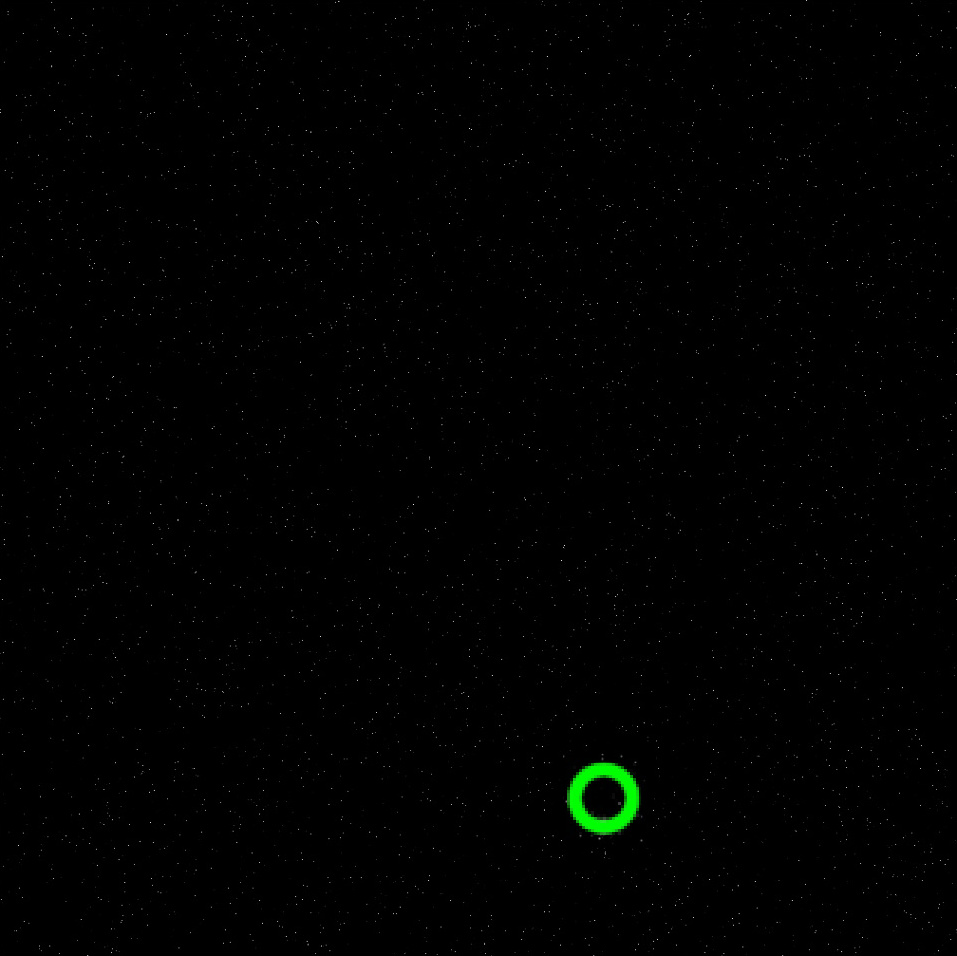
\includegraphics[width=\textwidth]{blob-dog/a1-180.0-18.0.jpg}
        \caption{\label{fig:ngc4147-dog} NGC 4147 (A1)}
    \end{subfigure}
    \begin{subfigure}[b]{0.33\textwidth}
        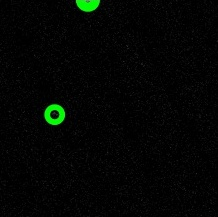
\includegraphics[width=\textwidth]{blob-dog/a1-228.0--2.0.jpg}
        \caption{\label{fig:palomar5-and-M5} Palomar 5 + M5 (A1)}
    \end{subfigure}
\end{figure}

\begin{figure}[H]\ContinuedFloat{}
    \centering
    \begin{subfigure}[b]{0.33\textwidth}
        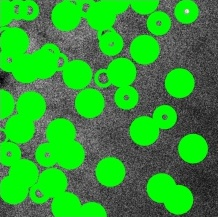
\includegraphics[width=\textwidth]{blob-dog/a2-295.0-15.0.jpg}
        \caption{\label{fig:M71-dog-4b4} M71 (A2: $\SI{4.0}{\degree}\times\SI{4.0}{\degree}$)}
    \end{subfigure}
    \begin{subfigure}[b]{0.33\textwidth}
        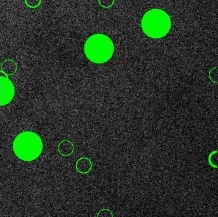
\includegraphics[width=\textwidth]{blob-dog/a2-297.0-17.0.jpg}
        \caption{\label{fig:M71-dog-2b2} M71 (A2: $\SI{2.0}{\degree}\times\SI{2.0}{\degree}$)}
    \end{subfigure}
\end{figure}

\begin{figure}[H]\ContinuedFloat{}
    \centering
    \begin{subfigure}[b]{0.33\textwidth}
        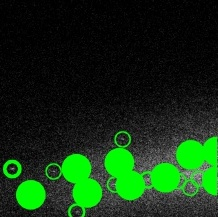
\includegraphics[width=\textwidth]{blob-dog/a3-8.0--74.0.jpg}
        \caption{\label{fig:small-magellanic-cloud}Small Magellanic Cloud (A3)}
    \end{subfigure}
    \begin{subfigure}[b]{0.33\textwidth}
        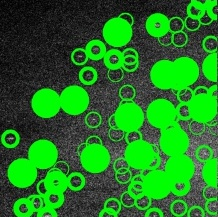
\includegraphics[width=\textwidth]{blob-dog/a3-72.0--70.0.jpg}
        \caption{\label{fig:large-magellanic-cloud}Large Magellanic Cloud (A3)}
    \end{subfigure}
\end{figure}

\begin{figure}[H]\ContinuedFloat{}
    \centering
    \begin{subfigure}[b]{0.33\textwidth}
        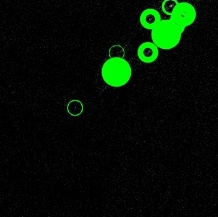
\includegraphics[width=\textwidth]{blob-dog/a4-8.0-38.0.jpg}
        \caption{\label{fig:andromeda}Andromeda Galaxy (A4)}
    \end{subfigure}
    \begin{subfigure}[b]{0.33\textwidth}
        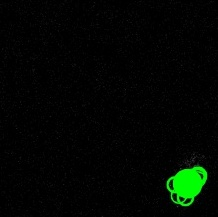
\includegraphics[width=\textwidth]{blob-dog/a4-20.0-30.0.jpg}
        \caption{\label{fig:triangulum}Triangulum Galaxy (A4)}
    \end{subfigure}

    \caption{\label{fig:dog-examples} Interesting Examples of the Blobs Found by \blobdog{}}
\end{figure}
The rasters in Area 1 (Figures \ref{fig:ngc4147-dog} and
\ref{fig:palomar5-and-M5}) show GCs that stand out visibly against their dark
stellar background. These blobs are easily found and identified even in the
scenario for M5 where the GC is only partially contained within the raster. The
rasters in Area 2 (Figures \ref{fig:M71-dog-4b4} and \ref{fig:M71-dog-2b2}) both
show the same region containing the GC M71. This GC is highlighted by \blobdog{}
across both rasterization schemes but at different scales. Additionally, it is
evident that the many smaller blobs identified in Figure~\ref{fig:M71-dog-2b2}
are not present in Figure~\ref{fig:M71-dog-4b4}. The rasters in Area 3 (Figures
\ref{fig:small-magellanic-cloud} and \ref{fig:large-magellanic-cloud}) show the
bright and busy Magellanic Clouds. No GCs are present in the Small Magellanic
Cloud shown in Figure~\ref{fig:small-magellanic-cloud}. Nevertheless, it is
still a busy area with many blobs being identified. The raster containing the
Large Magellanic Cloud contains four GCs (NGC 1696, NGC 1756, NGC 1786, and NGC
1795). While these GCs are identified in
Figure~\ref{fig:large-magellanic-cloud}, it is difficult to distinguish them due
to the amount of other blobs that are also highlighted. The rasters in Area 4
(Figure \ref{fig:andromeda} and \ref{fig:triangulum}) contain the Andromeda
Galaxy and the Triangulum Galaxy. These galaxies are identified as many smaller
blobs rather than a single continuous blob.

It is evident from the plots in Figure~\ref{fig:dog-examples} that \blobdog{} is
able to identify blobs across a wide range of scenarios. The results in Area 2:
$\SI{4.0}{\degree}\times\SI{4.0}{\degree}$ and the Magellanic Clouds reveal that
\blobdog{} is more responsive in bright busy areas. This behavior is beneficial
as brighter areas containing many stars are more likely to contain clusters.
Additionally, the difference in the blob detection between A2:
$\SI{2.0}{\degree}\times\SI{2.0}{\degree}$ and A2:
$\SI{4.0}{\degree}\times\SI{4.0}{\degree}$ reveals that the rasterization scheme
directly influences the results of \blobdog{}. Thus, more research should be
performed on identifying any possible parametric relationship between the
$B_{\text{threshold}}$ and the size of the rasters generated by the
rasterization scheme.

\newpage
\paragraph{Why are rasters containing known GCs filtered out at $B_{\text{threshold}} = 0.2$?}\paragraphnewline{}
\blobdog{} fails to identify all known GCs and filters away some rasters
containing known GCs. Table~\ref{tb:not-found-GCs} lists these GCs and provides
additional information to aid with identifying a trend underlying these
failures.
\begin{table}[H]
    \centering
    \caption{Known GCs that are Not Detected with $B_{\text{threshold}} = 0.2$}
    \label{tb:not-found-GCs}
    \begin{tabular}{lL{0.7\linewidth}}
        \toprule
        \multicolumn{2}{c}{Area 1}                                                                                                                                                                               \\
        \midrule
        Koposov 1    & A low-luminosity GC with a distance of \SI{48.3}{\kilo\parsec}~\cite{Koposov2007}.                                                                                                        \\
        Palomar 3    & A distant GC at \SI{96}{\kilo\parsec} with an apparent magnitude of \num{14.26}~\cite{Sharina2018}.                                                                                       \\
        Palomar 4    & A distant GC at \SI{109}{\kilo\parsec} with an apparent magnitude of \num{15.65}~\cite{listGC}.                                                                                           \\
        GCI 38       & A distant GC at \SI{74.7}{\kilo\parsec} with an apparent magnitude of \num{74.7}~\cite{listGC}.                                                                                           \\
        Willman 1    & An ultra low-luminosity GC with a distance of \SI{38}{\kilo\parsec} but with a very low brightness corresponding to an apparent magnitude of \num{15.2}~\cite{Willman2011}.\vspace{1.0em} \\
        \toprule
        \multicolumn{2}{c}{Area 3}                                                                                                                                                                               \\
        \midrule
        Arp Madore 1 & A very distant GC at \SI{123.3}{\kilo\parsec}~\cite{Arp-Madore-1}.                                                                                                                        \\
        \bottomrule
    \end{tabular}
\end{table}
All of these GCs that were not maintained are either very distant, have a
low-luminosity, or manifest both of these attributes. It is these factors that
lead to \blobdog{} failing to identify these clusters. This becomes apparent
visually when considering Figure~\ref{fig:missing-known-gcs-figure}.
\begin{figure}[H]
    \centering
    \begin{subfigure}[b]{0.32\textwidth}
        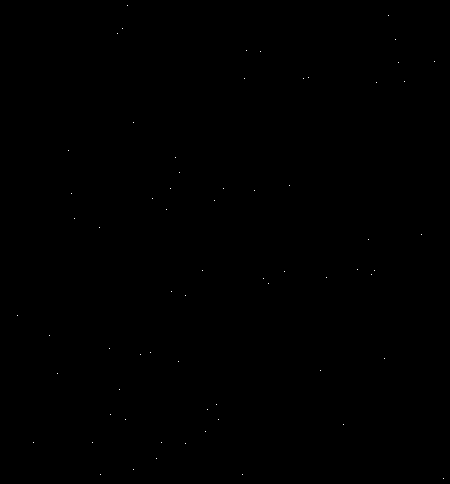
\includegraphics[width=\textwidth]{blob-dog/Koposov-1-scatter.png}
        \caption{\label{fig:koposov1} Koposov 1 (A1)}
    \end{subfigure}
    \begin{subfigure}[b]{0.32\textwidth}
        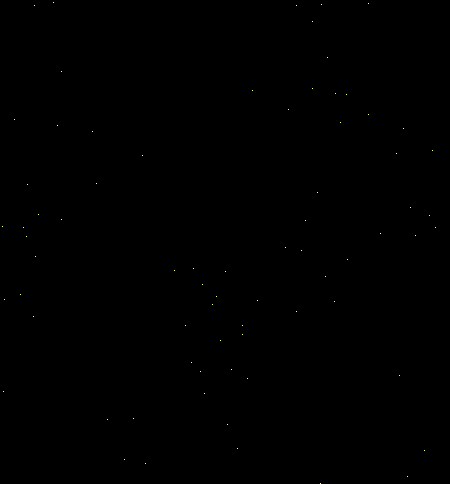
\includegraphics[width=\textwidth]{blob-dog/Palomar-3-scatter.png}
        \caption{\label{fig:palomar3} Palomar 3 (A1)}
    \end{subfigure}
    \begin{subfigure}[b]{0.32\textwidth}
        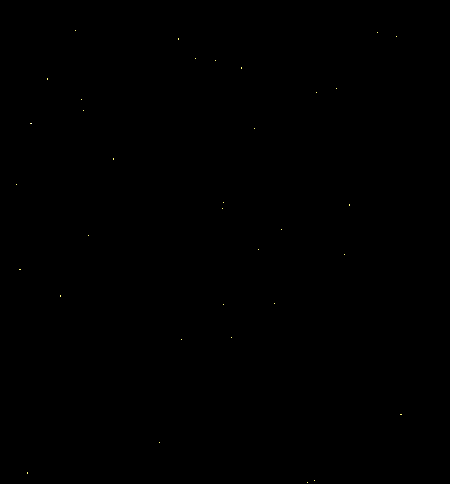
\includegraphics[width=\textwidth]{blob-dog/Palomar-4-scatter.png}
        \caption{\label{fig:palomar4} Palomar 4 (A1)}
    \end{subfigure}
\end{figure}

\begin{figure}[H]\ContinuedFloat{}
    \centering
    \begin{subfigure}[b]{0.32\textwidth}
        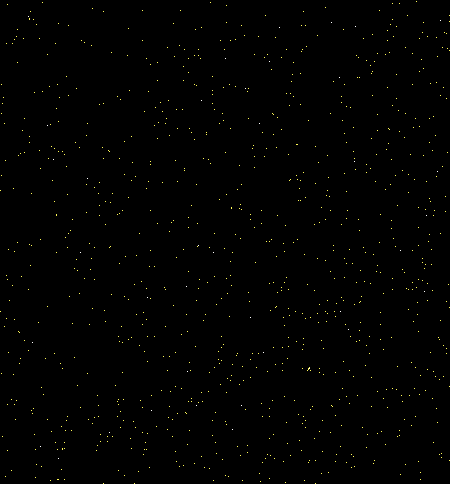
\includegraphics[width=\textwidth]{blob-dog/GCI-38-scatter.png}
        \caption{\label{fig:gci38} GCI 38 (A1)}
    \end{subfigure}
    \begin{subfigure}[b]{0.32\textwidth}
        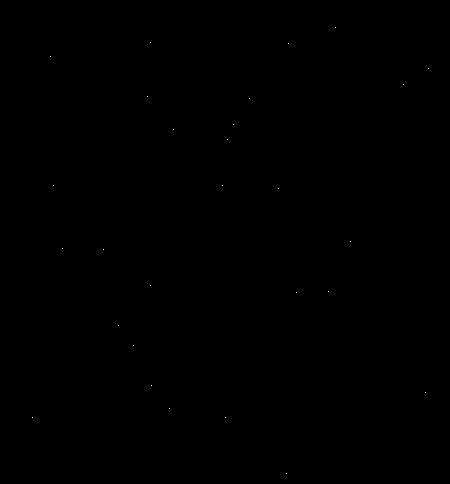
\includegraphics[width=\textwidth]{blob-dog/Willman-1-scatter.png}
        \caption{\label{fig:willman1} Willman 1 (A1)}
    \end{subfigure}
    \begin{subfigure}[b]{0.32\textwidth}
        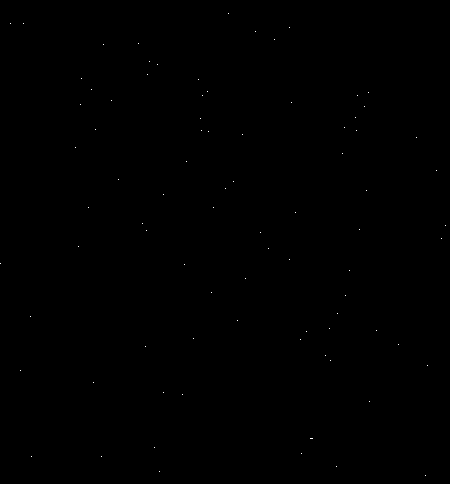
\includegraphics[width=\textwidth]{blob-dog/AM1-scatter.png}
        \caption{\label{fig:am1} Arp Madore (A3)}
    \end{subfigure}

    \caption{\label{fig:missing-known-gcs-figure} Known GCs Not Detected with $B_{\text{threshold}} = 0.2$}
\end{figure}
These GCs are barely visible or correspond with a very small blob (which would
then be discarded by the $B_{\text{threshold}} = 0.2$). It might be feasible to
resolve this by reducing the $B_{\text{threshold}}$ further. In addition, it may
be possible to make use of an alternate rasterization scheme which also
rasterizes across the distance. It would then be possible to
augment the rasters that are further away to better account for these distant
clusters at the cost of accuracy.

\paragraph{What would be the optimal $B_{\text{threshold}}$?}\paragraphnewline{}
\blobdog{} filters away $\SI{85}{\percent}$ of the rasters with a
$B_{\text{threshold}}$ of 0.2, while maintaining $\SI{80}{\percent}$ of the
known GCs. In ideal circumstances \blobdog{} would filter away many empty
rasters while still maintaining every raster containing a GC. Through the
testing performed in Section~\ref{sec:results-DoG}, it is evident that if an
optimal $B_{\text{threshold}}$ were to exist within the rasterization scheme
that was tested, it must lie between \SIrange{0.1}{0.2}{}. However, it is
possible that there is no $B_{\text{threshold}}$ which is able to maintain all
known GCs while still filtering away a majority of the rasters. Further
experimentation is required to test this.

\paragraph{How could \blobdog{} be improved?}\paragraphnewline{}
It is important to identify the relationship between the $B_{\text{threshold}}$
and the size of the rasters generated by the rasterization scheme. Furthermore,
the information provided by \blobdog{} could be used to provide better direction
to the Ant Colony algorithm. The locations of the blobs that were identified by
\blobdog{} could be used to provide the initial weights for the stars processed
by the Ant Colony. Thus, the initial generation of ants would be predisposed to
evaluate the regions containing those blobs.

In addition, the possibility of rasterizing in RA, Dec, as well as distance
should be evaluated. By rasterizing across distance as well, it may be possible
to enhance the rasters that are further away to better capture distant
low-luminosity clusters.

\blobdog{} is unable to account for distance in its results. This is in contrast
to the clustering algorithm which is able to classify multiple clusters
overlapping in RA and Dec. In the work by Mohammadi et al.~\cite{Mohammadi},
\blobdog{} was used as a post-processing step. If the rasterization is applied
across distance, this raises an interesting proposition for the use of
\blobdog{} in place of the gravitational clustering algorithm. For this final
step, \blobdog{} would be applied across RA and Dec with the luminosity for each
pixel being determined by the pheromone value of the star at that pixel. An example of \blobdog{} being applied as a post-processing mechanism may be seen in Figure~\ref{fig:mag-and-pher-based-DoG}.
\begin{figure}[H]
    \centering
    \begin{subfigure}[b]{0.49\textwidth}
        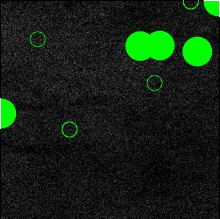
\includegraphics[width=\textwidth, height=\textwidth]{./figures/blob-dog/a4-0.0-58.0-magnitude-based-blobs.jpg}
        \caption{Magnitude based}
        \label{fig:mag-based}
    \end{subfigure}
    \begin{subfigure}[b]{0.49\textwidth}
        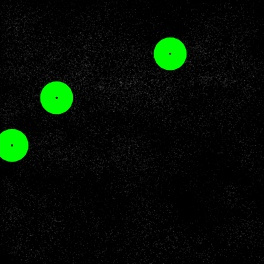
\includegraphics[width=\textwidth,height=\textwidth]{./figures/blob-dog/a4-0.0-58.0-pheromone-based-blobs.jpg}
        \caption{Pheromone based}
        \label{fig:pher-based}
    \end{subfigure}
    \caption{Blobs Identified by \blobdog{} In the Same Raster Under Different Parameters}
    \label{fig:mag-and-pher-based-DoG}
\end{figure}
As may be seen in this figure, the results of \blobdog{} when applied on the
absolute magnitude of the stars within the raster are very different to the
results when it is applied to the pheromone values of the stars within the
raster. In this instance, \blobdog{} is able to precisely identify the pheromone
clusters left by the Ant Colony. This highlights its potential as a mechanism to
cluster pheromone values. Incorporating this step would result in the pipeline
being as follows:
\begin{enumerate}
    \item Rasterize based on RA, Dec, and Distance.
    \item Apply \blobdog{} on the rasters based on their apparent magnitude.
    \item Generate the pheromone maps using the Ant Colony algorithm.
    \item Apply \blobdog{} on the pheromone values.
\end{enumerate}
Since \blobdog{} operates with a lower time complexity than the clustering
algorithm, this reformulation may provide sufficient results while operating
substantially faster.

\newpage
\section{\label{sec:eval-ant}Density Mapping Via the Ant Colony}

\paragraph{What is the behavior displayed by the Ant Colony algorithm?}\paragraphnewline{}
\noindent To examine the behavior of the Ant Colony algorithm, results for
various rasters across the areas are displayed in
Figure~\ref{fig:scatterplot-heatmaps}. The rasters that are examined are the
same as those that were used for the evaluation of the behavior of \blobdog{}.
To compare the distribution of the stars across the rasters against the network
substructure discovered by the Ant Colony algorithm, the stellar distribution
heat-maps of the rasters (indicated by $\dagger$) are positioned alongside the
pheromone heat-maps (indicated by $\ddagger$).

\begin{figure}[H]
    \centering
    \begin{subfigure}[b]{0.241\textwidth}
        \centering
        \captionsetup{justification=centering,format=hang}
        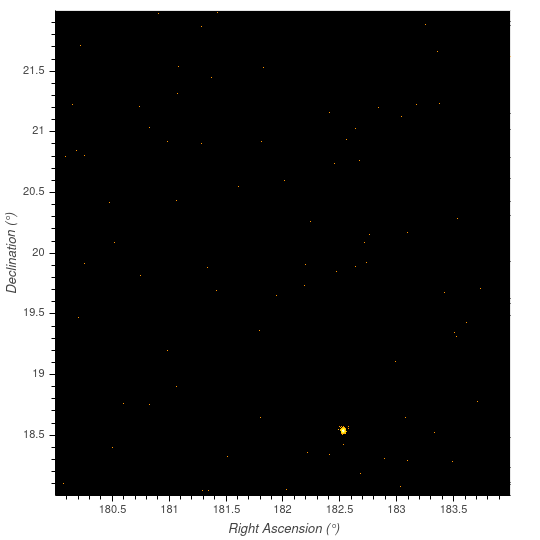
\includegraphics[width=0.95\textwidth, height=0.92\textwidth]{heatmaps/scatter-a1-180.0-18.0-ngc4147.png}
        \caption{\label{fig:scatter-ngc4147} NGC 4147~(A1)$^{\dagger}$ \phantom{abc def ghi}}
    \end{subfigure}
    \begin{subfigure}[b]{0.241\textwidth}
        \centering
        \captionsetup{justification=centering,format=hang}
        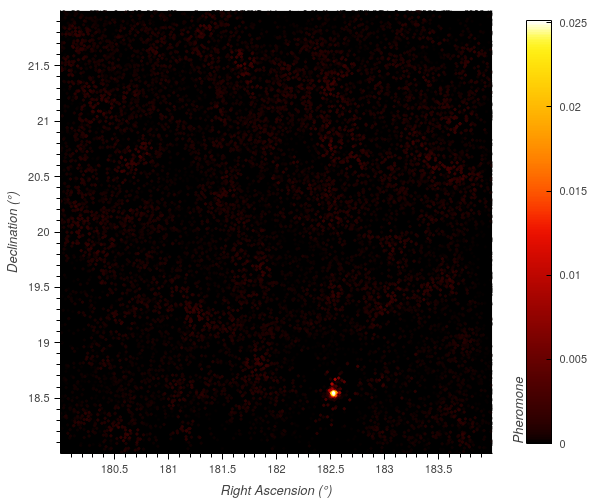
\includegraphics[width=1.1\textwidth, height=0.92\textwidth]{heatmaps/evaluation-ant/pheromone-map-a1-180.0-18.0-run-02.png}
        \caption{\label{fig:heat-ngc4147} NGC 4147~(A1)$^{\ddagger}$ \phantom{abc def ghi}}
    \end{subfigure}
    \hspace{0.3em}
    \begin{subfigure}[b]{0.241\textwidth}
        \centering
        \captionsetup{justification=centering,format=hang}
        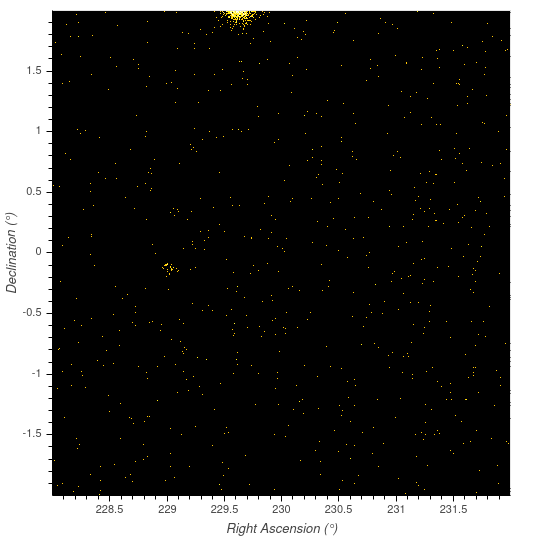
\includegraphics[width=0.95\textwidth, height=0.92\textwidth]{heatmaps/scatter-a1-palomar5+m5.png}
        \caption{\label{fig:scatter-palomar5} Palomar 5 + M5~(A1)$^{\dagger}$}
    \end{subfigure}
    \begin{subfigure}[b]{0.241\textwidth}
        \centering
        \captionsetup{justification=centering,format=hang}
        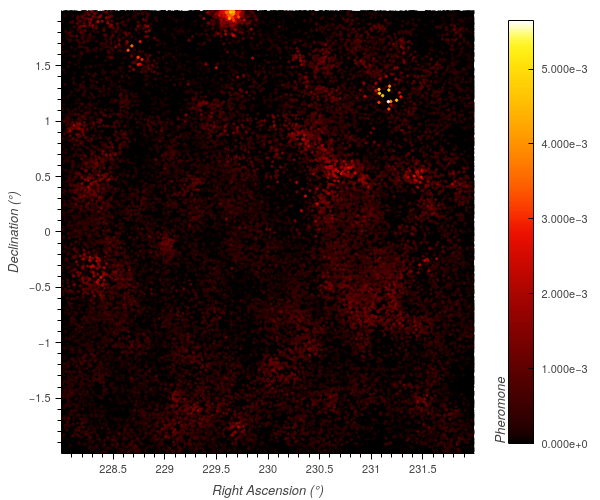
\includegraphics[width=1.14\textwidth, height=0.92\textwidth]{heatmaps/evaluation-ant/pheromone-map-a1-228.0--2.0-run-05.png}
        \caption{\label{fig:heat-palomar5} Palomar 5 + M5~(A1)$^{\ddagger}$}
    \end{subfigure}
    \begin{subfigure}[b]{0.241\textwidth}
        \centering
        \captionsetup{justification=centering,format=hang}
        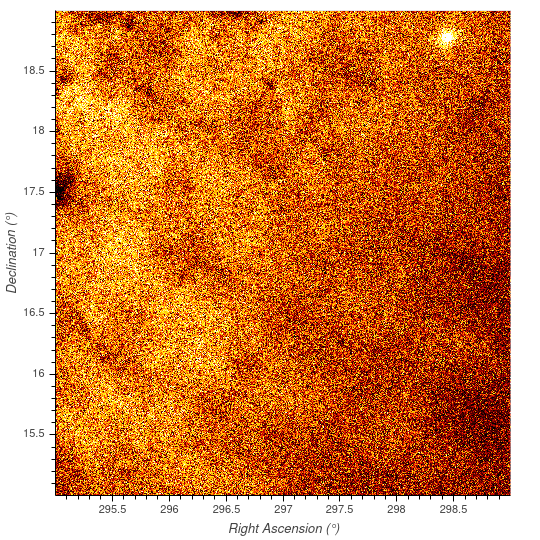
\includegraphics[width=0.95\textwidth, height=0.92\textwidth]{heatmaps/scatter-a2-gc-4x4.png}
        \caption{\label{fig:scatter-M71-dog-4b4}M71~(A2: $\SI{4.0}{\degree}\times\SI{4.0}{\degree}$)$^{\dagger}$}
    \end{subfigure}
    \begin{subfigure}[b]{0.241\textwidth}
        \centering
        \captionsetup{justification=centering,format=hang}
        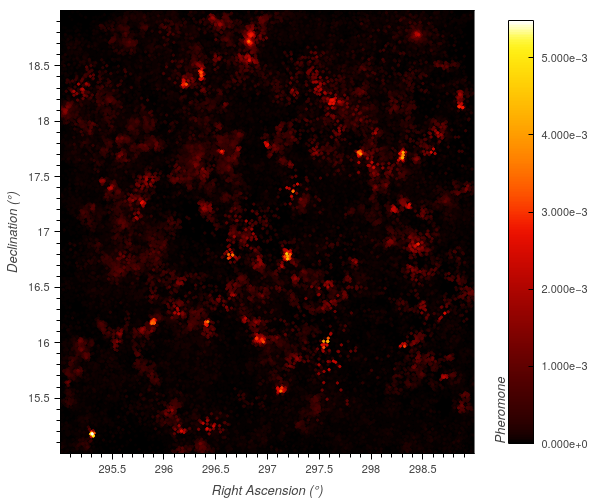
\includegraphics[width=1.14\textwidth, height=0.92\textwidth]{heatmaps/evaluation-ant/pheromone-map-a2-4x4-295.0-15.0-run-03.png}
        \caption{\label{fig:heat-M71-dog-4b4}M71~(A2: $\SI{4.0}{\degree}\times\SI{4.0}{\degree}$)$^{\ddagger}$}
    \end{subfigure}
    \hspace{0.3em}
    \begin{subfigure}[b]{0.241\textwidth}
        \centering
        \captionsetup{justification=centering,format=hang}
        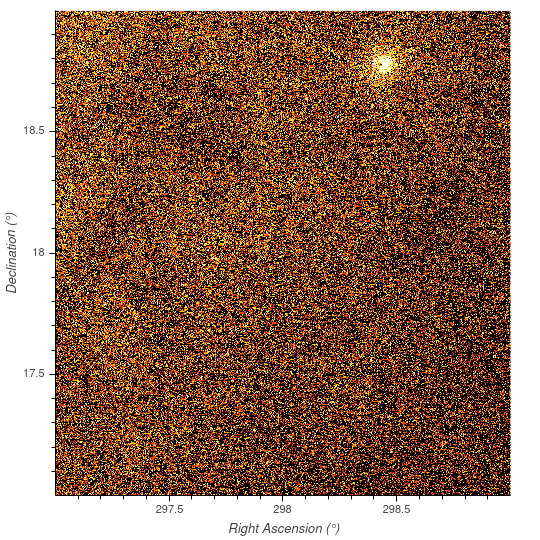
\includegraphics[width=0.95\textwidth, height=0.92\textwidth]{heatmaps/scatter-a2-gc-2x2.png}
        \caption{\label{fig:scatter-M71-dog-2b2}M71~(A2: $\SI{2.0}{\degree}\times\SI{2.0}{\degree}$)$^{\dagger}$}
    \end{subfigure}
    \begin{subfigure}[b]{0.241\textwidth}
        \centering
        \captionsetup{justification=centering,format=hang}
        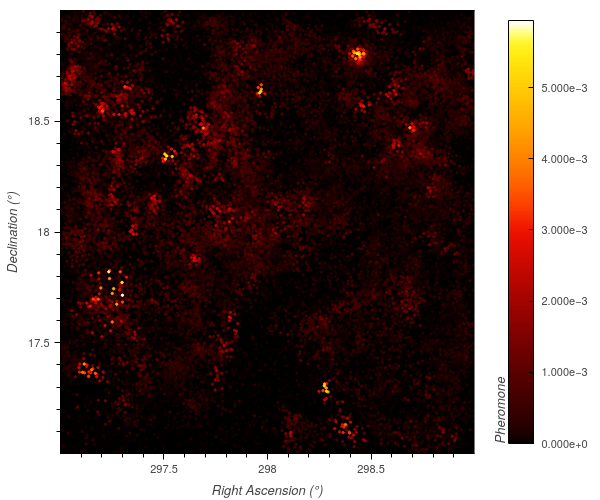
\includegraphics[width=1.14\textwidth, height=0.92\textwidth]{heatmaps/evaluation-ant/pheromone-map-a2-297.0-17.0-run-01.png}
        \caption{\label{fig:heat-m71-dog-2b2}M71~(A2: $\SI{2.0}{\degree}\times\SI{2.0}{\degree}$)$^{\ddagger}$}
    \end{subfigure}

    \begin{subfigure}[b]{0.241\textwidth}
        \centering
        \captionsetup{justification=centering,format=hang}
        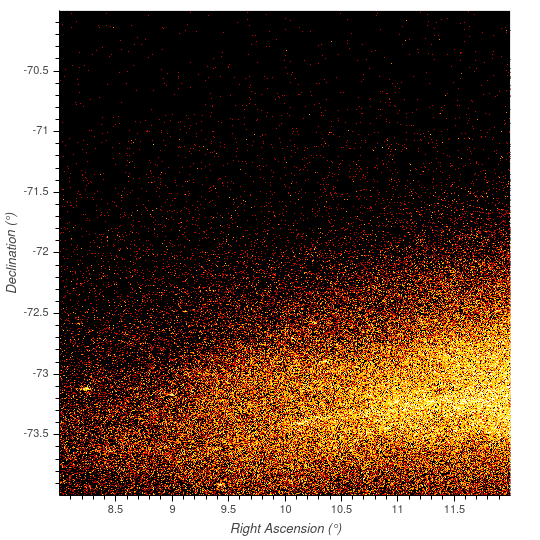
\includegraphics[width=0.95\textwidth, height=0.92\textwidth]{heatmaps/scatter-a3-gc-small-MC.png}
        \caption{\label{fig:scatter-small-magellanic-cloud}Small Magellanic Cloud~(A3)$^{\dagger}$}
    \end{subfigure}
    \begin{subfigure}[b]{0.241\textwidth}
        \centering
        \captionsetup{justification=centering,format=hang}
        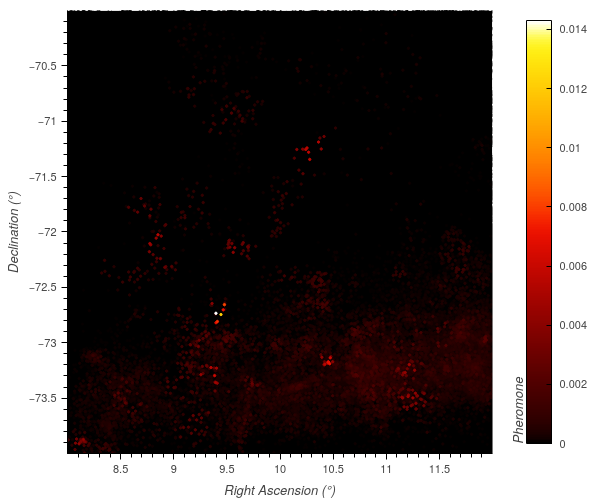
\includegraphics[width=1.1\textwidth, height=0.92\textwidth]{heatmaps/evaluation-ant/pheromone-map-a3-8.0--74.0-run-04.png}
        \caption{\label{fig:heat-small-magellanic-cloud}Small Magellanic Cloud~(A3)$^{\ddagger}$}
    \end{subfigure}
    \hspace{0.3em}
    \begin{subfigure}[b]{0.241\textwidth}
        \centering
        \captionsetup{justification=centering,format=hang}
        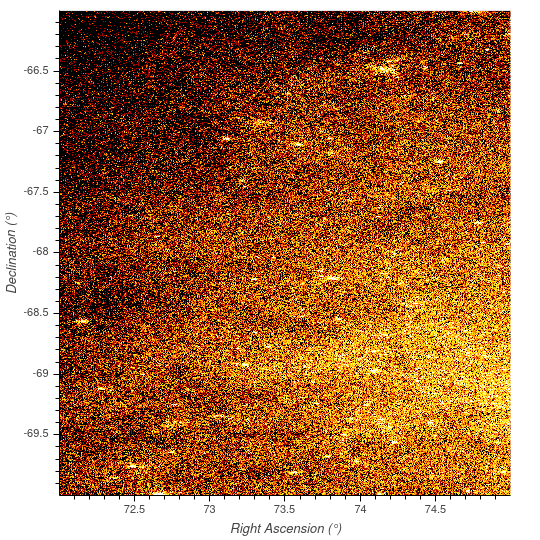
\includegraphics[width=0.95\textwidth, height=0.92\textwidth]{heatmaps/scatter-a3-gc-large-MC.png}
        \caption{\label{fig:scatter-large-magellanic-cloud}Large Magellanic Cloud~(A3)$^{\dagger}$}
    \end{subfigure}
    \begin{subfigure}[b]{0.241\textwidth}
        \centering
        \captionsetup{justification=centering,format=hang}
        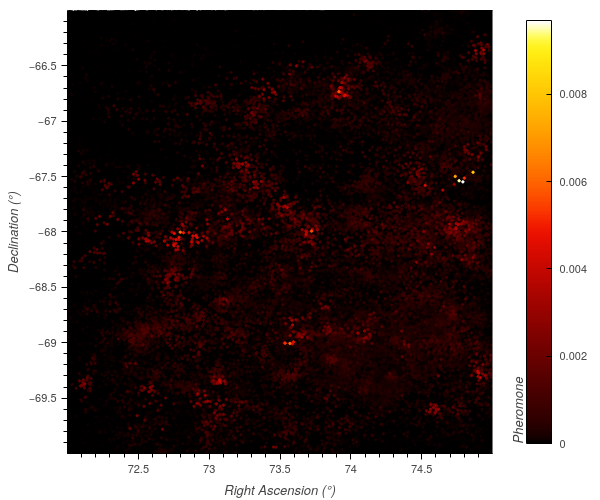
\includegraphics[width=1.1\textwidth, height=0.92\textwidth]{heatmaps/evaluation-ant/pheromone-map-a3-72.0--70.0-run-01.png}
        \caption{\label{fig:heat-large-magellanic-cloud}Large Magellanic Cloud~(A3)$^{\ddagger}$}
    \end{subfigure}

    \begin{subfigure}[b]{0.241\textwidth}
        \centering
        \captionsetup{justification=centering,format=hang}
        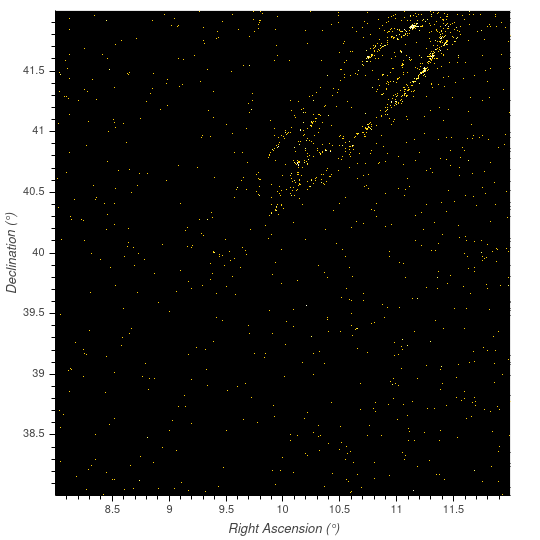
\includegraphics[width=0.95\textwidth, height=0.92\textwidth]{heatmaps/scatter-a4-andromeda.png}
        \caption{\label{fig:scatter-andromeda}Andromeda Galaxy~(A4)$^{\dagger}$}
    \end{subfigure}
    \begin{subfigure}[b]{0.241\textwidth}
        \centering
        \captionsetup{justification=centering,format=hang}
        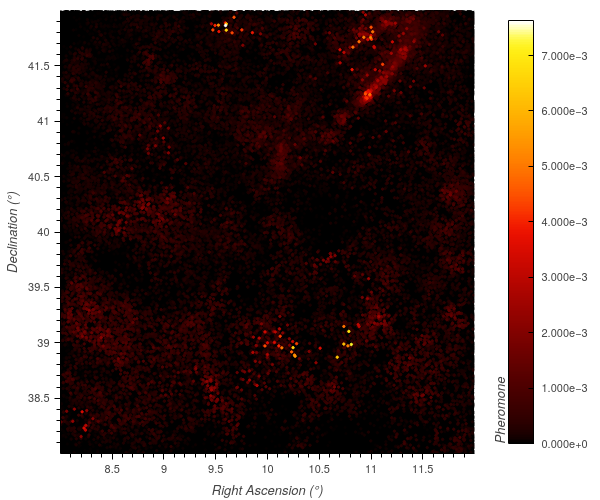
\includegraphics[width=1.14\textwidth, height=0.92\textwidth]{heatmaps/evaluation-ant/pheromone-map-a4-8.0-38.0-run-05.png}
        \caption{\label{fig:heat-andromeda}Andromeda Galaxy~(A4)$^{\ddagger}$}
    \end{subfigure}
    \hspace{0.3em}
    \begin{subfigure}[b]{0.241\textwidth}
        \centering
        \captionsetup{justification=centering,format=hang}
        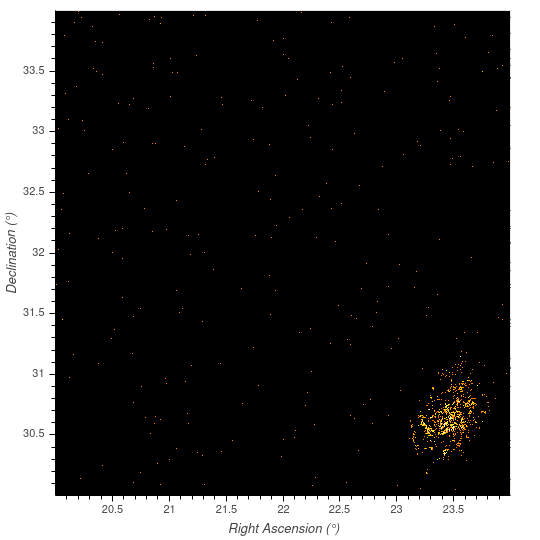
\includegraphics[width=0.95\textwidth, height=0.92\textwidth]{heatmaps/scatter-a4-triangulum.png}
        \caption{\label{fig:scatter-triangulum}Triangulum Galaxy~(A4)$^{\dagger}$}
    \end{subfigure}
    \begin{subfigure}[b]{0.241\textwidth}
        \centering
        \captionsetup{justification=centering,format=hang}
        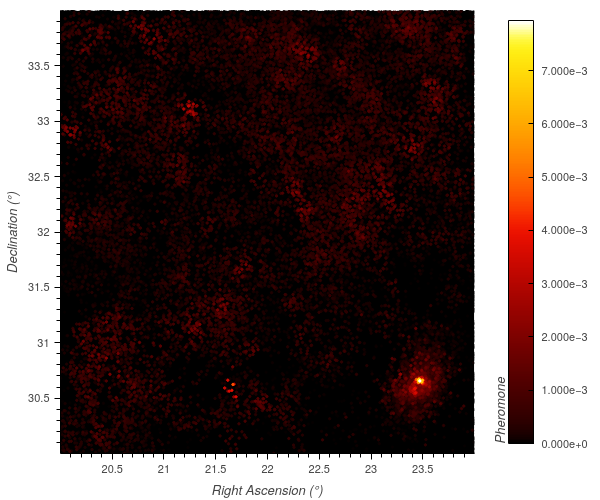
\includegraphics[width=1.14\textwidth, height=0.92\textwidth]{heatmaps/evaluation-ant/pheromone-map-a4-20.0-30.0-run-05.png}
        \caption{\label{fig:heat-triangulum}Triangulum Galaxy~(A4)$^{\ddagger}$}
    \end{subfigure}

    \caption{\label{fig:scatterplot-heatmaps} Stellar Distribution Heat-maps ($\dagger$) vs. Pheromone Heat-maps ($\ddagger$) for Various Rasters}
\end{figure}

The algorithm functioning as intended should result in pheromone mappings honed
in on stellar clusters and other dense regions. From the plots of the rasters in
Area 1 and Area 4, it is evident that the algorithm works well at identifying
concentrated clusters of stars surrounded by regions of very low concentration.
The structure of these rasters is directly observable in the density map
uncovered by the Ant Colony. The plots for Area 1 demonstrate the ability of the
Ant Colony algorithm to highlight the location of GCs through an increased
concentration of pheromone values. Visually, this corresponds to the focused
bright spot present in the pheromone heat-map of the rasters. For the plots of
Area 4, the pheromone heat-maps show larger bright smudges corresponding to the
nearby galaxies contained within those rasters. These pheromone mappings are
less intense but still stand out, clearly formed in the shape of the galaxies at
hand. For Area 1 and 4, the algorithm is able to distinctly identify these
clusters. However, the results for the other areas are less definitive.

For Area 2: $\SI{2.0}{\degree}\times\SI{2.0}{\degree}$ it is able to highlight the GC
contained within the upper-right corner of the raster, but it does so with many
other less relevant regions also being highlighted. This is taken to the extreme
with Area 2: $\SI{4.0}{\degree}\times\SI{4.0}{\degree}$ which does not clearly
identify the GC at all. The difference in these outcomes is due to the disparity
in the number of stars contained within both rasters. As Area 2:
$\SI{2.0}{\degree}\times\SI{2.0}{\degree}$ contains less stars, the connected
structure that this GC demonstrates, represents an increased proportion of the
total substructure. Thus, the ants are more likely to gather within the GC to
pool their pheromone values than in Area 2:
$\SI{4.0}{\degree}\times\SI{4.0}{\degree}$. Both rasters present a busy starscape and
it seems that the ants are being spread too thin to have their pheromone values
be reliably identified by the clustering phase that follows.

The plots for Area 3 focus on the rasters containing the Magellanic Clouds.
Figure~\ref{fig:heat-small-magellanic-cloud} is of the Small Magellanic Cloud
and has no GCs present, while Figure~\ref{fig:heat-large-magellanic-cloud} shows
the Large Magellanic Cloud which contains the four GCs: NGC 1696, NGC 1756, NGC
1786, and NGC 1795. These GCs were not identified in the results of the final
pipeline. The pheromone values across the rasters containing these GCs are
distributed erratically by the ants without sufficient concentration. As a
result, no cluster gets singled out by the clustering phase. However, the full
pipeline does identify many clusters contained within Area 3. These clusters are
primarily on the fringes in rasters that do not contain many stars. Many of them
are contained within the Dec bound of $\SI{-90.0}{\degree}$ and
$\SI{-86.0}{\degree}$. These rasters represent the least busy regions in Area 3.

Table~\ref{tb:Nstars-in-reffig} lists the number of stars contained within each
raster that was examined and presents additional statistics on the pheromone
values associated with that raster.
\begin{table}[H]
    \centering
    \caption{Visualization of the Star and Pheromone ($\mathbf{f}$) Information of Each Raster in Figure~\ref{fig:scatterplot-heatmaps}.}
    \label{tb:Nstars-in-reffig}
    \begin{tabular}{l@{\hspace{0.35\tabcolsep}} l r c c}
        \toprule
        \multicolumn{2}{l}{Figure}            & \multicolumn{1}{c}{$N_{\text{stars}}$}               & $\mathbf{f}_{\text{max}}$ & $\mathbf{f}_{\text{mean}}$                                                                                                                                                                                                      \\
        \midrule
        \ref{fig:heat-ngc4147}                & NGC 4147 (A1)                                        & \num{26778}               & \num[round-mode=figures, round-precision=4, fixed-exponent=2, scientific-notation=true]{0.02512871666666667}  & \num[round-mode=figures, round-precision=4, fixed-exponent=2, scientific-notation=true]{0.00030600848084248473} \\
        \ref{fig:heat-palomar5}               & Palomar 5 + M5 (A1)                                  & \num{76687}               & \num[round-mode=figures, round-precision=4, fixed-exponent=2, scientific-notation=true]{0.005648536666666666} & \num[round-mode=figures, round-precision=4, fixed-exponent=2, scientific-notation=true]{0.00010685377052173344} \\
        \ref{fig:heat-M71-dog-4b4}            & M71 (A2: $\SI{4.0}{\degree}\times\SI{4.0}{\degree}$) & \num{3246820}             & \num[round-mode=figures, round-precision=4, fixed-exponent=2, scientific-notation=true]{0.00548187}           & \num[round-mode=figures, round-precision=4, fixed-exponent=2, scientific-notation=true]{2.5237910016584272e-06} \\
        \ref{fig:heat-m71-dog-2b2}            & M71 (A2: $\SI{2.0}{\degree}\times\SI{2.0}{\degree}$) & \num{771759}              & \num[round-mode=figures, round-precision=4, fixed-exponent=2, scientific-notation=true]{0.005943506666666667} & \num[round-mode=figures, round-precision=4, fixed-exponent=2, scientific-notation=true]{1.0617686479849747e-05} \\
        \ref{fig:heat-small-magellanic-cloud} & Small Magellanic Cloud (A3)                          & \num{301721}              & \num[round-mode=figures, round-precision=4, fixed-exponent=2, scientific-notation=true]{0.014302903333333335} & \num[round-mode=figures, round-precision=4, fixed-exponent=2, scientific-notation=true]{2.715851763715874e-05}  \\
        \ref{fig:heat-large-magellanic-cloud} & Large Magellanic Cloud (A3)                          & \num{576494}              & \num[round-mode=figures, round-precision=4, fixed-exponent=2, scientific-notation=true]{0.00969327}           & \num[round-mode=figures, round-precision=4, fixed-exponent=2, scientific-notation=true]{1.4214016277709483e-05} \\
        \ref{fig:heat-andromeda}              & Andromeda Galaxy (A4)                                & \num{97875}               & \num[round-mode=figures, round-precision=4, fixed-exponent=2, scientific-notation=true]{0.00763254}           & \num[round-mode=figures, round-precision=4, fixed-exponent=2, scientific-notation=true]{8.372204444444661e-05}  \\
        \ref{fig:heat-triangulum}             & Triangulum Galaxy (A4)                               & \num{66763}               & \num[round-mode=figures, round-precision=4, fixed-exponent=2, scientific-notation=true]{0.007941336666666667} & \num[round-mode=figures, round-precision=4, fixed-exponent=2, scientific-notation=true]{0.00012273707143178251} \\
        \bottomrule
    \end{tabular}
\end{table}

What can be observed in this table is that the mean pheromone value
($\mathbf{f}_{\text{mean}}$) from the rasters of Area 2 and Area 3 are much
smaller than the values of Area 1 and Area 4. This again emphasizes the
relationship of the number of stars and the behavior of the Ant Colony algorithm
expressed with the pheromone values.

Ultimately, the Ant Colony algorithm demonstrates effective behavior in specific
circumstances (namely rasters with a large variation in stellar density across
the raster). However, the algorithm requires further optimization to function as
effectively on rasters with a more uniform distribution and those containing
many stars.

\paragraph{What are the shortcomings of the Ant Colony algorithm?}\paragraphnewline{}
\noindent
There are two major shortcomings in the implementation of the Ant Colony
algorithm. Firstly, it is possible that the ants are unable to evaluate their
environment sufficiently. This is evident from the inability of the Ant Colony
to successfully identify any clusters in Area
2:~$\SI{4.0}{\degree}\times\SI{4.0}{\degree}$. The configuration of the
parameters of the Ant Colony play the primary factor in determining the scale at
which the Ant Colony is able to successfully operate. It is crucial to identify
this relationship between these parameters and the properties of the rasters
being evaluated given the central nature of the Ant Colony algorithm to the
functioning of the whole pipeline.

Secondly, the Ant Colony algorithm computes the Euclidean Distance between stars
in RA, Dec, and Distance. However, this assumes that the basis units of each of
these axes are uniform. While this holds between RA and Dec as they are in the
same unit, it does not hold with distance. It may be possible to determine some
relationship between the RA, Dec, and Distance which operates functionally.

\paragraph{How could the Ant Colony algorithm be improved?}\paragraphnewline{}
\noindent
Two main suggestions for improving the Ant Colony algorithm are:
\begin{enumerate}
    \item Determining the relationship between the configuration constants for the
          Ant Colony algorithm and the characteristics of the input rasters. The aim
          would be to identify a method of dynamically setting these constants based on
          the raster. This information could then also be forwarded alongside the
          pheromone results to the clustering algorithm.
    \item As with the same improvement mentioned for \blobdog{}, introducing a
          rasterization scheme which also cuts across distance. This would make it easier
          for the Ant Colony algorithm to control the number of stars being processed per
          raster and thereby improve the uniformity of the behavior of the Ant Colony.
\end{enumerate}

\section{\label{sec:eval-clustering}Gravitational Clustering Based on Pheromone Mapping}

\paragraph{What is the behavior displayed by the Gravitational Clustering algorithm? }\paragraphnewline{}
To explore the behavior of the clustering algorithm, plots are generated to
compare the distribution of pheromone values across a raster against the
resulting clustering. Figure~\ref{fig:eval-clustering-2d-ngc4147} shows such a
comparison for the raster containing the GC NGC 4147.

\begin{figure}[H]
    \centering
    \begin{subfigure}[b]{0.49\textwidth}
        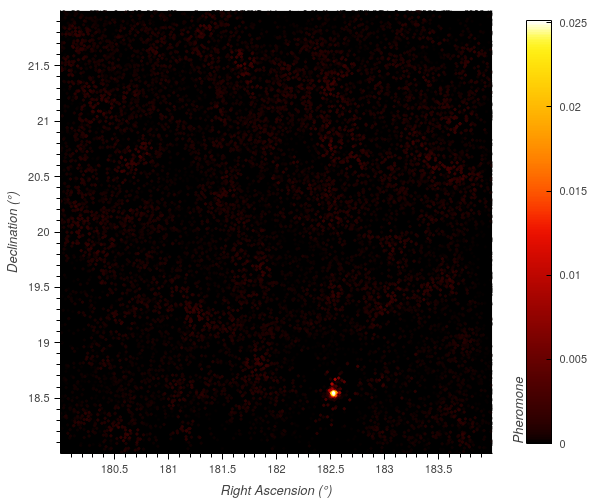
\includegraphics[height=0.8\textwidth, width=\textwidth]{{evaluation/a1-180.0-18.0-run-02-2d-pheromone.png}}
        \caption{\label{fig:eval-clustering-2d-ngc4147-pheromone}Pheromone Heat-map}
    \end{subfigure}
    \begin{subfigure}[b]{0.49\textwidth}
        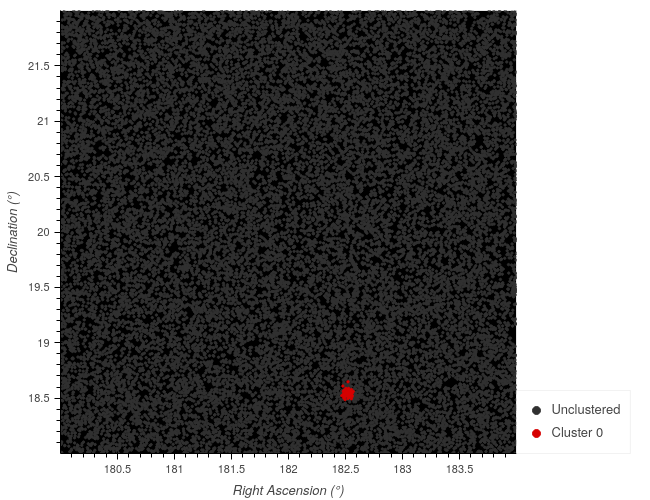
\includegraphics[height=0.8\textwidth, width=\textwidth]{{evaluation/a1-180.0-18.0-run-02-2d-cluster.png}}
        \caption{\label{fig:eval-clustering-2d-ngc4147-cluster}Cluster Plot}
    \end{subfigure}
    \caption{\label{fig:eval-clustering-2d-ngc4147}2D Plots of NGC 4147}
\end{figure}
\vspace{-0.5em}

The distribution of the pheromone values presented in
Figure~\ref{fig:eval-clustering-2d-ngc4147-pheromone} are precisely represented
in the clustering presented in
Figure~\ref{fig:eval-clustering-2d-ngc4147-cluster}. These plots are effective
at showcasing the clustering across RA and Dec. However, unlike \blobdog{}, the
Ant Colony algorithm and the Gravitational Clustering algorithm operate by
taking into account a third distance dimension. The comparison showing this
distance dimension may be seen in Figure~\ref{fig:eval-clustering-3d-ngc4147}.

\begin{figure}[H]
    \centering
    \begin{subfigure}[b]{0.49\textwidth}
        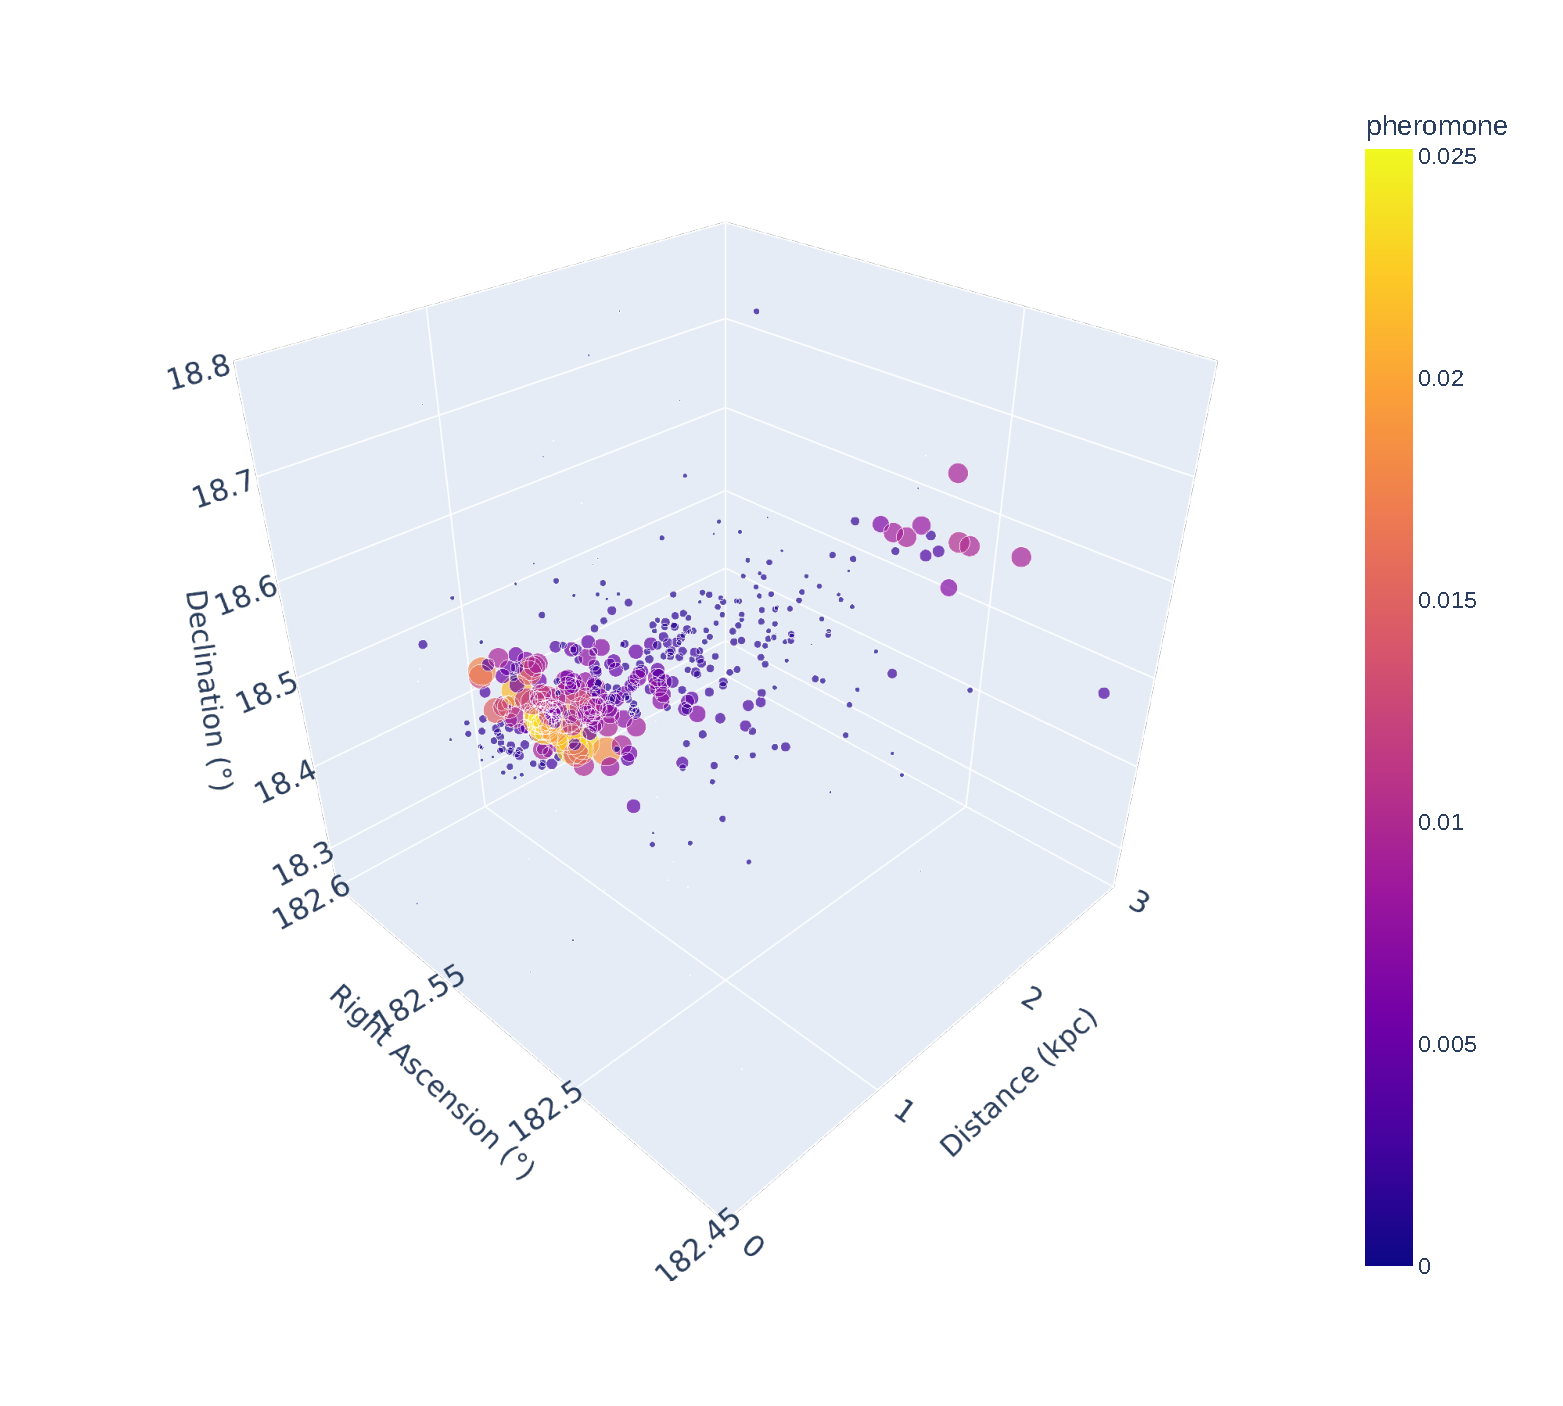
\includegraphics[width=\textwidth]{{evaluation/a1-180.0-18.0-run-02-3d-pheromone.pdf}}
        \caption{Pheromone Heat-map}
        \label{fig:ph-3d-18}
    \end{subfigure}
    \begin{subfigure}[b]{0.49\textwidth}
        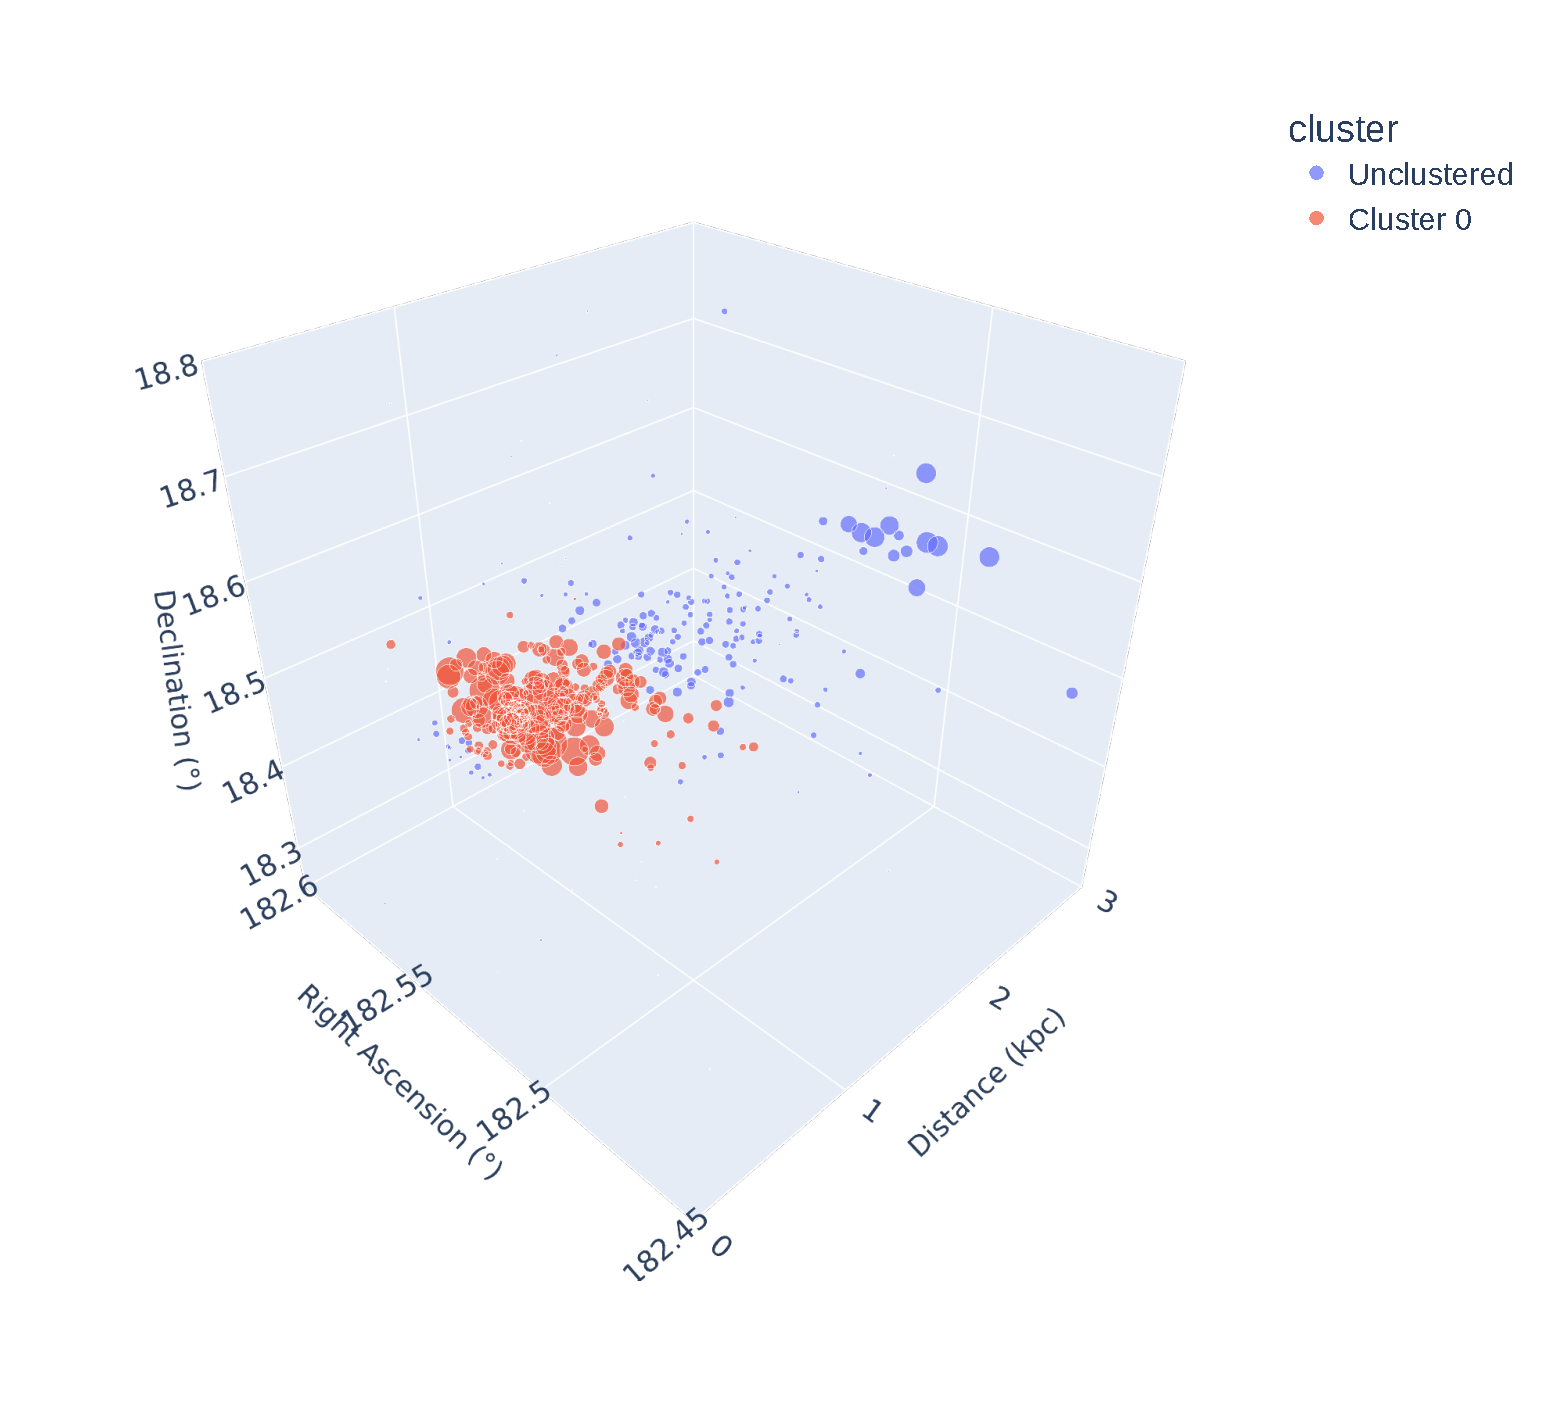
\includegraphics[width=\textwidth]{{evaluation/a1-180.0-18.0-run-02-3d-cluster.pdf}}
        \caption{Cluster Plot}
        \label{fig:cp-3d-18}
    \end{subfigure}
    \caption{3D Plots of NGC 4147}
    \label{fig:eval-clustering-3d-ngc4147}
\end{figure}

Figure~\ref{fig:eval-clustering-3d-ngc4147} shows 3D scatterplots zoomed-in on
the area around the cluster. The size of each point in the scatterplot
corresponds to the magnitude of the pheromone value (as does the color in the
case of the pheromone heat-map). It is clear from these figures, that the center
of the cluster contains the stars with the highest pheromone values.
Additionally, a separate group with high pheromone values may be observed within
the distance of \SI{2}{\kilo\parsec} to \SI{3}{\kilo\parsec}. The main grouping evidently contains more than 100 stars whereas this other group contains less than 100 stars and is not classified as a cluster.

It is interesting to consider the scenario where the clustering algorithm does
identify multiple clusters within the same raster. This is case for the raster
containing the GC NGC 5024 and the 2D plot of the comparison between the
pheromones values for this raster and the clustering may be seen in
Figure~\ref{fig:eval-clustering-2d-ngc5024}.

\begin{figure}[H]
    \centering
    \begin{subfigure}[b]{0.49\textwidth}
        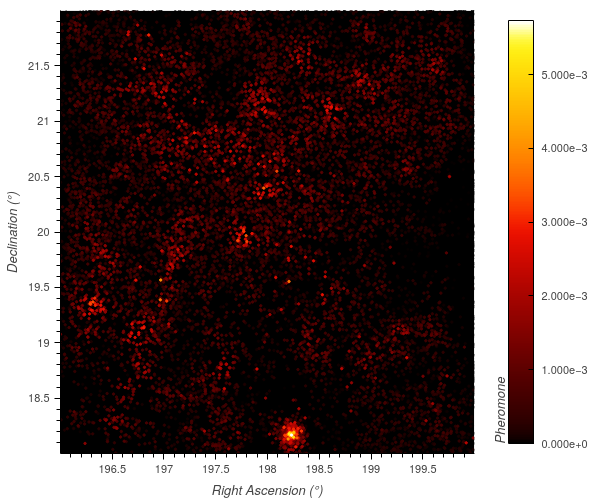
\includegraphics[height=0.8\textwidth, width=\textwidth]{{evaluation/a1-196.0-18.0-run-01-2d-pheromone.png}}
        \caption{Pheromone Heat-map}
    \end{subfigure}
    \begin{subfigure}[b]{0.49\textwidth}
        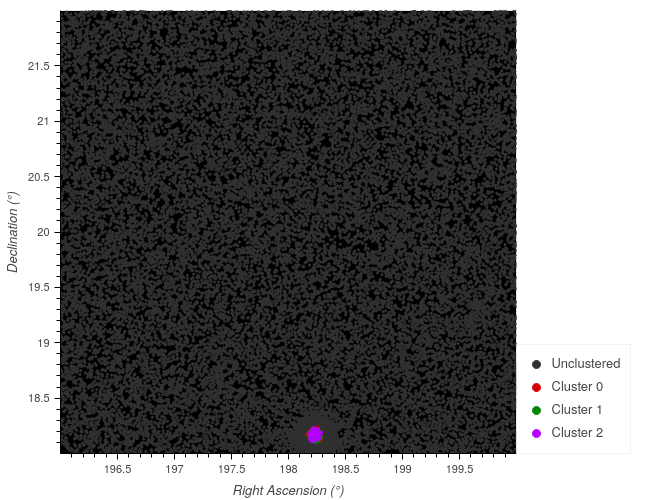
\includegraphics[height=0.8\textwidth, width=\textwidth]{{evaluation/a1-196.0-18.0-run-01-2d-cluster.png}}
        \caption{Cluster Plot}
    \end{subfigure}
    \caption{2D Plots of NGC 5024}
    \label{fig:eval-clustering-2d-ngc5024}
\end{figure}

In Figure~\ref{fig:eval-clustering-2d-ngc5024}, only the results for
\textit{Cluster 2} seem apparent. This is because the clusters overlap in RA and
Dec and this is confirmed when considering the plots in
Figure~\ref{fig:eval-clustering-3d-ngc5024}.
\begin{figure}[H]
    \centering
    \begin{subfigure}[b]{0.49\textwidth}
        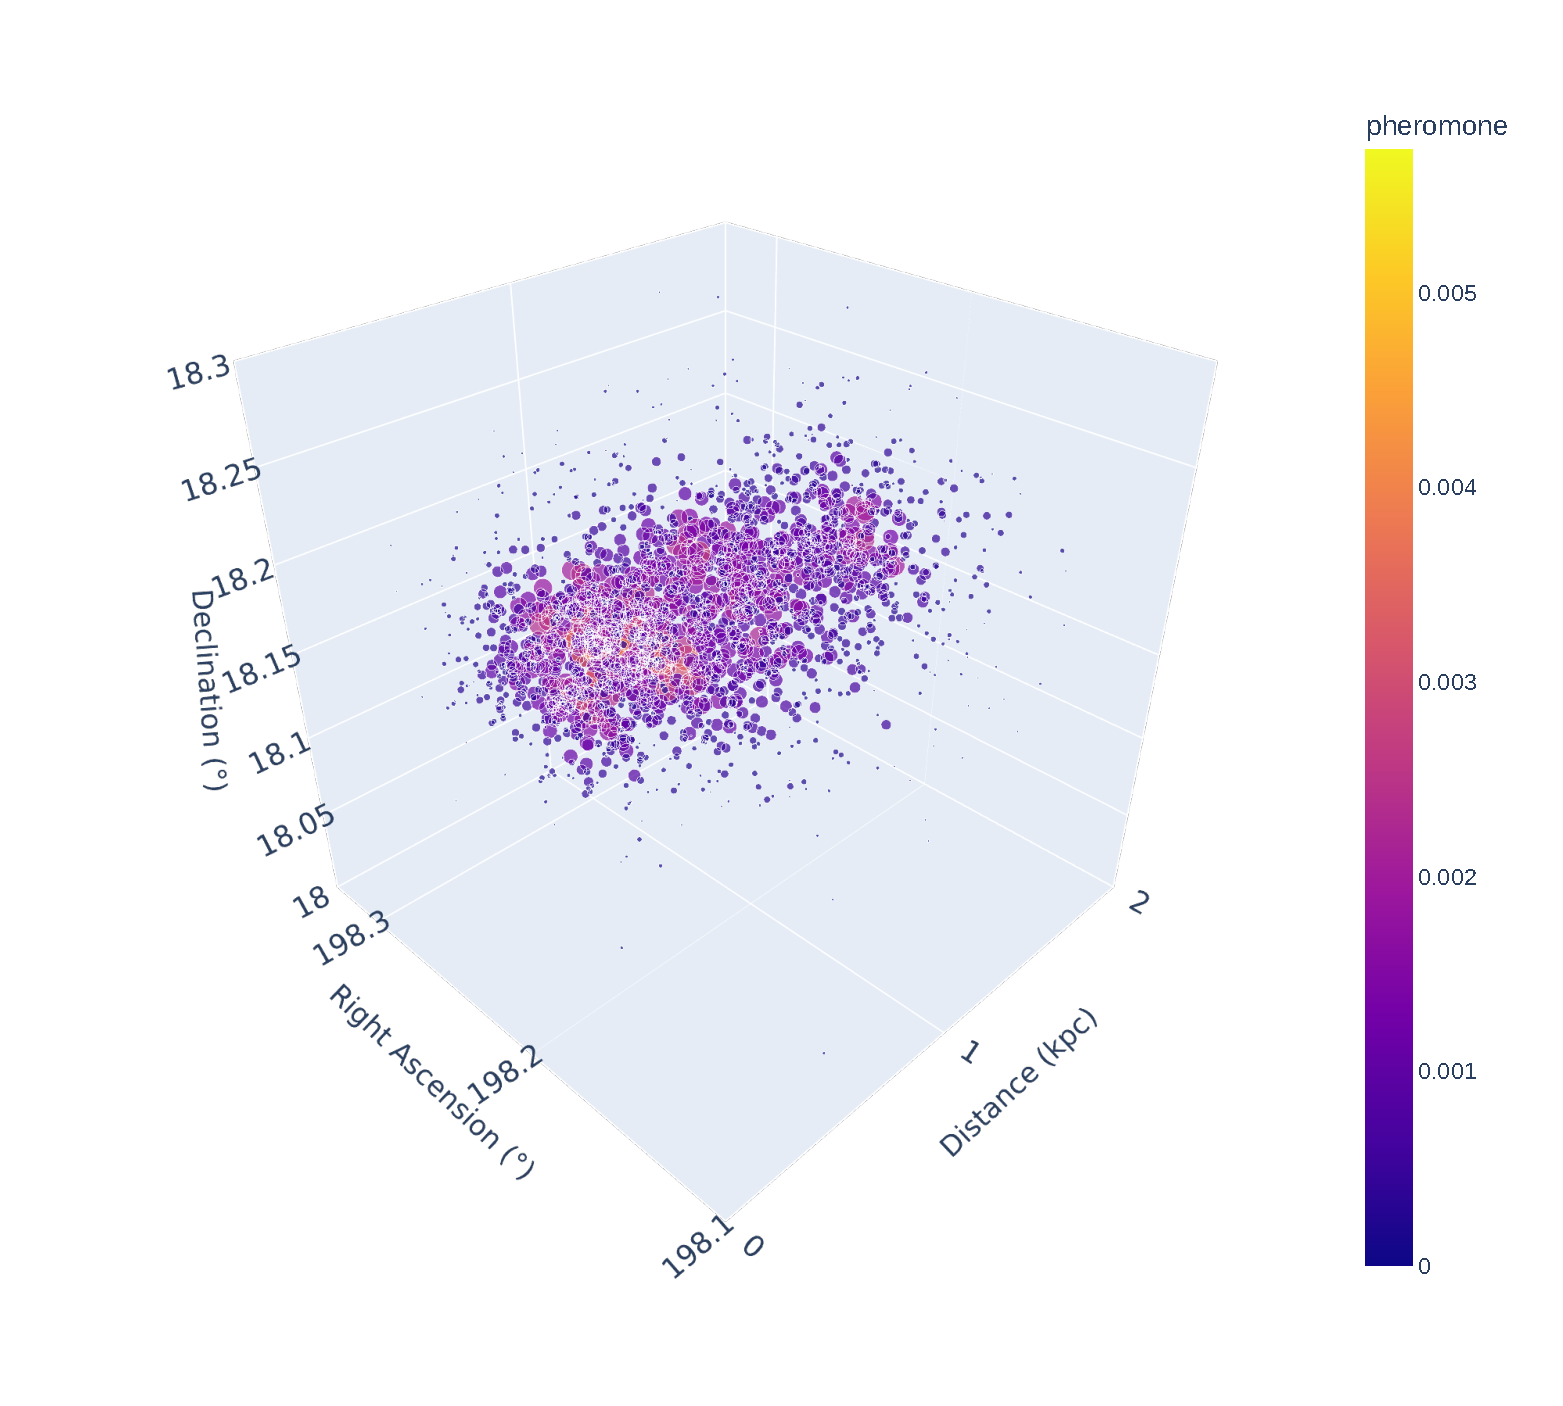
\includegraphics[width=\textwidth]{{evaluation/a1-196.0-18.0-run-01-3d-pheromone.pdf}}
        \caption{\label{fig:eval-clustering-3d-ngc5024-pheromone}Pheromone Heat-map}
    \end{subfigure}
    \begin{subfigure}[b]{0.49\textwidth}
        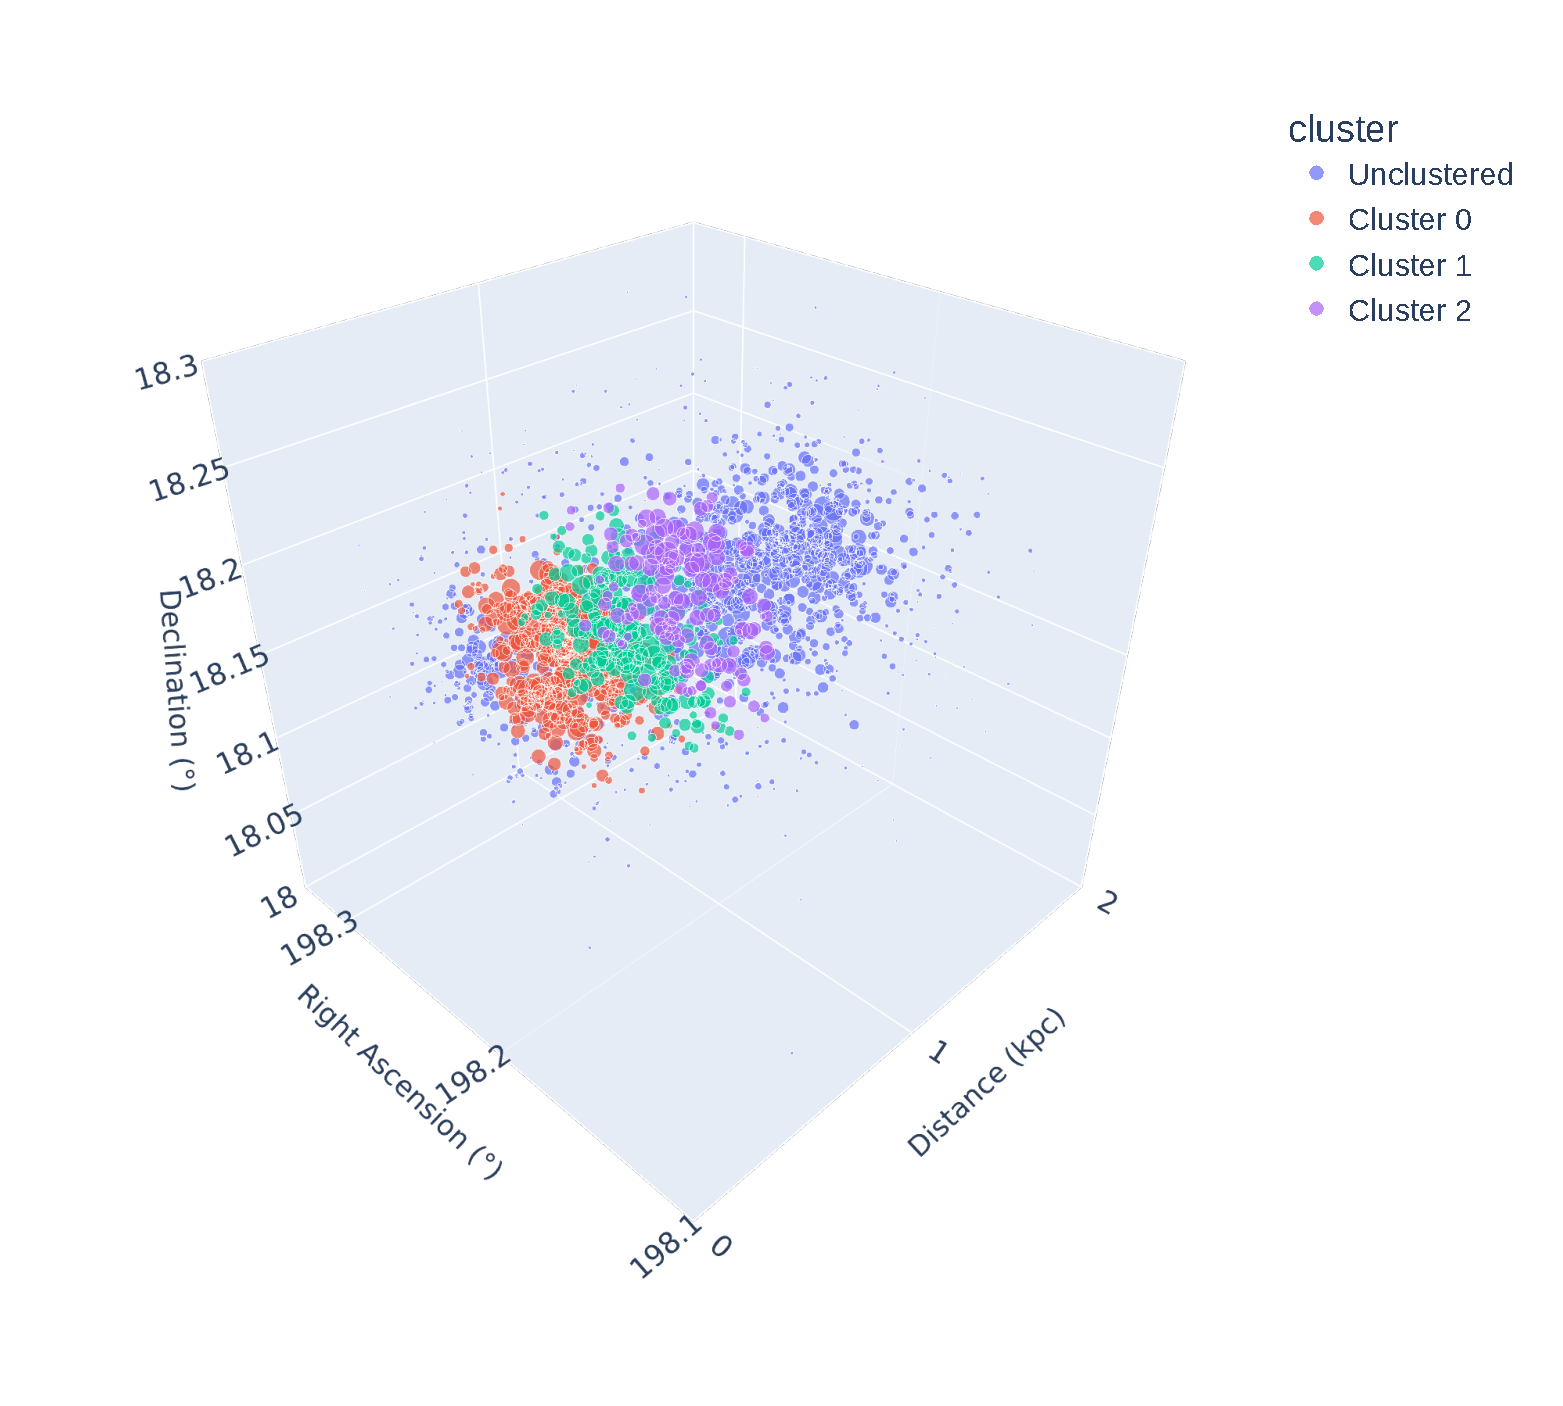
\includegraphics[width=\textwidth]{{evaluation/a1-196.0-18.0-run-01-3d-cluster.pdf}}
        \caption{\label{fig:eval-clustering-3d-ngc5024-cluster}Cluster Plot}
    \end{subfigure}
    \caption{\label{fig:eval-clustering-3d-ngc5024}3D Plots of NGC 5024}
\end{figure}

The pheromone values seem uniformly distributed over the zoomed-in range
displayed in Figure~\ref{fig:eval-clustering-3d-ngc5024-pheromone}. When
comparing this region to the region presented in
Figure~\ref{fig:eval-clustering-2d-ngc4147} there seem to be many more stars
present. Additionally, unlike Figure~\ref{fig:eval-clustering-2d-ngc4147} it is
hard to visually distinguish any sub-clusters across this range. These pheromone
values appear as a single agglomerate structure. However, the clustering
algorithm does distinguish this group into multiple clusters. It is evident from
Figure~\ref{fig:eval-clustering-3d-ngc5024-cluster} that the clustering
algorithm identifies 3 distinct clusters around the center of mass of the
pheromone values. These clusters appear as thin slices all in close proximity to
each other with no apparent unclustered regions interlacing them. This indicates
an issue in the behavior of the clustering algorithm.

\paragraph{What are the shortcomings of the Gravitational Clustering algorithm?}\paragraphnewline{}
From Figure~\ref{fig:eval-clustering-3d-ngc5024}, it becomes apparent that the
clustering algorithm functions well in RA and Dec but seems miscalibrated under
distance. This is due to the fact that the basis unit for RA, Dec, and distance
are treated as the same unit. Thus, a \ang{1.0} shift in RA or Dec is considered
equivalent to a \SI{1.0}{\kilo\parsec} shift in distance. However, in reality
this comparison is not physically sensible and it is evident from the results
that the relative scaling for these bases are inappropriate. This same issue
pervades the Ant Colony as well as it also makes use of Euclidean Distance.

Additionally, the fact that clusters are being split into multiple clusters under distance
means that the sizes of the resulting cluster are underestimated. The parameter
${N_{\text{GC}}}_{\text{min}}$ is set to a constant of 100. Thus, it is possible
that a cluster whose total number of stars is above 100 has been filtered away
as it was split into multiple clusters. This, likely explains why some clusters
were identified only in {\large $\nicefrac{4}{5}$} experiments. Instead of
making a binary decision, it would be practical to provide a continuous metric
describing the validity of a given cluster.

Finally, more experimentation is required to determine an optimal value for
$F_{\text{min attraction}}$. This evaluation should also consider possible
relationships between the properties of the raster and the constants that were
used in previous phases of the pipeline.

\paragraph{How could the Gravitational Clustering algorithm be improved?}\paragraphnewline{}
There are a number of possible improvements that could be considered for the Gravitational
Clustering algorithm:

\begin{enumerate}
    \item More testing must be done to determine any possible parametric relationships between the constants set in the previous phases of the pipeline and the constants used in the clustering phase.
    \item The Ant Colony algorithm and the Gravitational Clustering algorithm
          both make use of Euclidean Distance, which treats the scale of the basis units
          for RA, Dec, and Distance identically. However, the distance operates with
          different units to the RA and Dec and this results in miscalibration of the
          algorithm in considering the distance. This could be temporarily alleviated by
          special casing the distance metric in the computations or by evaluating another
          distance metric perhaps under a different geometric scheme (e.g. spherical
          coordinates).
    \item After the initial clusters have been formed, the clustering algorithm
          makes a binary decision based on the number of stars within the cluster. This
          decision determines whether or not that cluster should be classified as a valid
          cluster. This is mainly to remove small clusters that were formed containing
          very few stars (approaching one star). Instead, it would be appropriate to
          provide a continuous metric on the certainty of a given cluster being valid.
          This, step could also evaluate other properties such as metallicity. These metrics could also be used to differentiate between different cluster types.
\end{enumerate}
